Bien des techniques d'approximation d'EDPs d'évolution font intervenir à un moment la résolution d'une équation différentielle ordinaire (EDO
\footnote{On utilisera aussi le terme \textit{système dynamique}, même si en toute rigueur ce concept est un peu plus large.}),
c'est à dire une équation différentielle ne faisant intervenir qu'une seule variable de difénretiation (ici le temps). Nous commeçons donc cette section par rappeler 
quelques notions d'analyse et de simulation des EDOs\footnote{Pour nos besoins nous nous restreignons au EDO du premier ordre.}.\par

\begin{definition}[Équation différentielle ordinaire]
    Une équation différentielle ordinaire est une équation de la forme :
    \begin{align}
        u' &= f(u,t)\quad u : t \in \mathbb{R}^+ \mapsto u(t) \in \mathbb{R}^d\\\notag
        u(0)&=u_0.
    \end{align}
\end{definition}
%%%%%%%%%%%%%%%%%%%%%%%%%%%%%%%%%%%%%%%%%%%%%%%%%%%%%%%%%%%%%%%%%%%%%%%%    SCHEMA EXPLICITES ET IMPLCITES
\paragraph{Schémas explicites et implcites.}
L'approximation des EDO se fait grâce à des schéma numériques. Ceux-ci se divisent en deux catégories, les schéma explicites et les schéma implicite
\footnote{Nous présentons ici seulement les schéma à un pas et non pas les schémas multi-pas. Ce choix est fait en raison de la barrière de Dhalquist.}.
Dans ce qui suit on note $u^n$ l'approximation de la solution d'une EDO au pas de temps $n$, c'est à dire que donné un pas de discrétisation temporel $\Delta t$
l'objectif est d'avoir $u^n \approx u(t=n\Delta t)$.

\begin{definition}[Schéma explicite]
    Un schéma numérique est dit explicite si le pas de temps $n+1$ est obtenu grâce au pas de temps $n$, c'est à dire : 
    \begin{align}
        u^{n+1} = u^n + f(u^n ,\Delta t ).
    \end{align}
\end{definition}

\begin{definition}[Schéma implicite]
    Un schéma numérique est dit implicite si le pas de temps $n+1$ est obtenu grâce au pas de temps $n$ \textbf{et} $n+1$, c'est à dire : 
    \begin{align}
        u^{n+1} = u^n + + f(u^{n+1} ,\Delta t ).
    \end{align}
    Ainsi, une itétation d'un schéma implcite nécessite l'inversion d'un système linéaire ou non linéaire. 
\end{definition}
De fait une itéraiton implcite est souvent plus couteuse qu'une itération d'un schéma explicite
\footnote{En particulier si la dimension de la solution $d$ est grande.}. 
Cependant pour des raisons de stabilités les méthodes explicites peuvent nécessiter des pas de temps bien plus fin, et donc bien plus d'itérations.
Le choix entre méthode explicite et implcite dépend de bien des facteurs (du problème, du niveau de précision voulu, de la difficulté d'implémentation etc...)
c'est un enjeu central de la simulation numérique.
%%%%%%%%%%%%%%%%%%%%%%%%%%%%%%%%%%%%%%%%%%%%%%%%%%%%%%%%%%%%%%%%%%%%%%%%
\paragraph{Stabilité des schémas numériques}
Un schéma numérique d'ordre $p$ converge vers la solution exacte de l'EDO avec une erreur qui décroît asymptotiquement en $\Delta t^p$ lorsque le pas de temps diminue.
Cependant, cette convergence n'est garantie que si le schéma reste stable.
L'instabilité se manifeste par une divergence de la solution numérique : au-delà d'un pas de temps critique $\Delta t_0$, la norme de la solution discrète $\|u^n\|$ tend vers l'infini\footnote{Phénomène communément appelé "explosion" de la solution numérique.}.
Cette instabilité peut s'interpréter de deux manières complémentaires : d'un point de vue mathématique, le schéma se comporte comme une suite géométrique de raison $|r| > 1$ ; d'un point de vue physique, le schéma introduit artificiellement de l'énergie dans le système à chaque itération.
La contrainte de stabilité impose donc $\Delta t < \Delta t_0$. Lorsque ce seuil est très restrictif, la résolution de l'EDO nécessite un nombre important d'itérations, augmentant considérablement le coût calculatoire. 
Comme évoqué précédemment les méthodes explicites sont généralement plus bien sensibles à cette limitation que les méthodes implicites.
\begin{figure}[htbp]
    \centering
    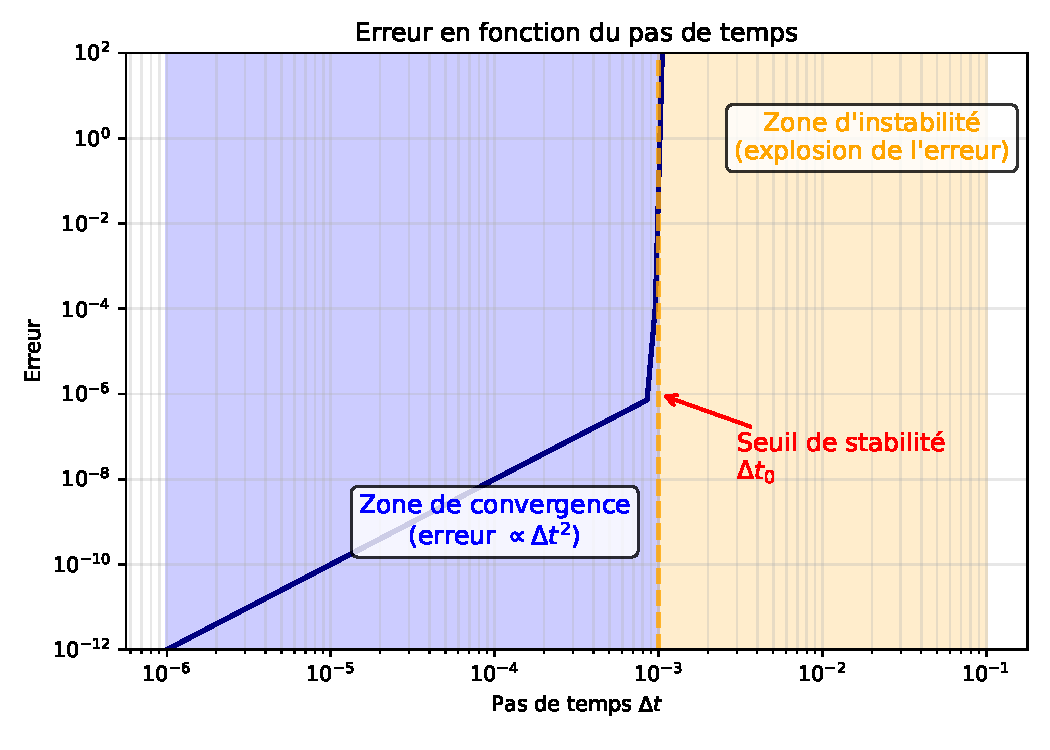
\includegraphics[width=0.8\textwidth]{media/3_/2_/exemple_satabilite.pdf}
    \caption{Exemple illustratif du comportement de l'erreur de l'approximation dans le ca d'un schéma d'ordre 2 avec une instabilité pour $\Delta t > 10^{-1}$.}
    \label{fig:stabilite_schema}
\end{figure}
\begin{definition}[Stabilité d'un schéma numérique]
    Un schéma numérique $n \mapsto u^n \in \mathbb{R}^d$ est stable si est seulement si :
    \begin{align}
        \Vert u^{n+1} \Vert \leq \Vert u^n \Vert.
    \end{align}
    Pour un schéma d'intégration et une ODE fixée, cette condition peut être vérifiée ou non en fonction de la valeur 
    du pas discrétisation $\Delta t$.
\end{definition}
La stabilité d'une méthode d'intégration d'EDO dépend entre autre de l'opérateur intervenant dans l'équation.
Un opérateur prompt à poser des problèmes de stabilité.
\begin{definition}[Problème raide]
    Un système dynamqiue, est dit raide si les méthodes explicites ne sont pas adaptées à sa résolution.
    En termes plus mathématiques le système 
    \begin{align}
    \frac{\text d u}{\text{d}t} = f(u,t) \quad u(t) \in \mathbb{R}^d \: \forall t\geq 0.
    \end{align}
    est dit raide si la jacobienne de $f$, $J_f$ possède de \text{grandes} valeurs propres négatives
    \footnote{Ici \textit{grand} est à comprendre au sens de \textit{grande aplitude devant d'autres valeurs propres}.}.
\end{definition}
En simplfiaint, si un opérateur est raide, il impose une condition de stabilité très restrictive aux méthodes explicites et 
force à choisir des méthodes implcites\footnote{La réalité est plus nuancée, nous le verrons.}.
\begin{exemple}[Équation de Dhalquist]
    Pour saisir de manière plus intuitive le concept de raideur, prenons le cas symple de l'équation de Dhalquist définissant le système suivant
    \footnote{C'est le cas le plus simple d'une valeur propre négative}:
    \begin{align}
        \frac{\text d u }{\text d t} &= - \lambda u,\quad \lambda > 0\\\notag
        u(t=0)&=u_0
    \end{align}
    La solution analytique est : $u(t) = u_0 e^{-\lambda t}$. Ainsi passé quelque $ 1/\lambda$ la dynamqiue du système est au point mort. 
    Grossièrement la dynamqiue digne d'intérêt du système se concentre entre $t=0$ et $t=\frac{10}{\lambda}$. 
    Au delà, $u(t>\frac{10}{\lambda}) = o(u_0)$, la dynamqiue est terminée.
    Ainsi le lecteur comprend aisément que si l'on souhaite simuler le comportement d'un tel système, il faut prendre des pas de temps petits devant $\vert \lambda \vert^{-1}$.
    Si $\lambda$ est de grande amplitude cela peut devenir très contraignant... Si l'on souhaite utiliser des méthodes explicites, c'est encore pire car la raideur du sysème 
    n'est plus un simple contrainte de précision mais de stabilité. En effet si l'on cherche à approximer le sysètme par un schéma d'Euler explicite, alors : 
    $U^{n+1} = U^n (1 - \lambda \Delta t)$ alors la contrainte de stabilité est $\Delta t \, \lambda < 1/2$ ce qui est contraignant si $\lambda$ est grand. 
    Si $\lambda = 10^5$ alors il faut avoir $\Delta t /approx 10^{-5}$ donc pour simuler le système entre $t=0$ et $t=1$ il faut cent-milles points !
    A l'inverse si l'on choisit un schéma d'Euler implicite: $u^{n+1} = u^n - \lambda \Delta t u^{n+1}$, alors la condition de stabilité devient : 
    $\Vert(1+\lambda \Delta t)^{-1}\Vert \leq 1$ ce qui est toujours vrai, quelque soit $- \lambda \in \mathbb{R}^-$, la raideur du système n'est pas un problème pour la méthode implicite.
    On comprend mieux la définition précédente \textit{Un système dynamqiue, est dit raide si les méthodes explicites ne sont pas adaptées à sa résolution.}
\end{exemple}
Il existe plusieurs type de stabilité comme la A-stabilité (méthode stable indépedemment de la raideur du problème), la L-stabilité (schéma amortissant les hautes fréquences),
par soucis de concision nous n'irons pas plus loins mais le lecteur intéressé se réfèrera à \cite{HairerAndWanner1}.